\section{Introduction}
\label{sec:intro}

Conversational agents such as Alexa, Siri, and Google Assistant should help users discover, learn, and retain novel factual information.
More generally, systems for conversational information-seeking should help users develop their information need, be mixed-initiative, incorporate user memory, and reason about the utility of retrieved information as a combined set~\citep{Radlinski2017ATF}.
We focus on a curiosity-driven, information-seeking scenario where a user starts a conversation with an assistant by asking an open-ended question and then drills down into interest areas (Figure~\ref{fig:example}).
\begin{figure}[t]
\centering
\begingroup
\addtolength\leftmargini{-5mm}
\begin{itemize}
    \setlength\itemsep{-1.25mm}
          \it
          \fontsize{10}{12}\selectfont
    \item[] U: <assistant wake-word>, tell me about Tahiti.
    \item[] A: It's the largest island in French Polynesia, near the center of the Pacific
    \item[] U: What is its history with France?
\end{itemize}
\endgroup
\caption{
    An example of information-seeking dialog that the \rover{} dataset aims to support.
    Assistants should answer user questions \emph{and} convey information that inspires meaningful followup questions.
}
\label{fig:example}
\end{figure}

In this setting, what policies should assistants pursue to maintain the user's interest in the topic?
Theories of human learning, such as Vygotsky's zone of proximal development, propose that learning novel information should be rooted in pre-existing knowledge and skills of the learner~\citep{chaiklin-03}.
Considering this, a good policy may give general information about Tahiti; a better policy would select information related to the user's knowledge (e.g., familiarity with France).
We hypothesize that engagement is correlated with policies that integrate a user's pre-existing knowledge, and test this through a large-scale, Wizard-of-Oz~(\woz{}) style collection~\citep{Kelley1984AnID,Wen2016ANE} that captures assistant policies, user reactions, and topically relevant entities that the user knows about.
The \rover{} dataset has \ndialogsfull{} English dialogs annotated with sentence-level knowledge grounding, the user's prior knowledge, dialog acts per message, and binary ratings per message.\footnote{
    Dataset and code at \dsurl{}.
}

\begin{figure}[t]
    \centering
    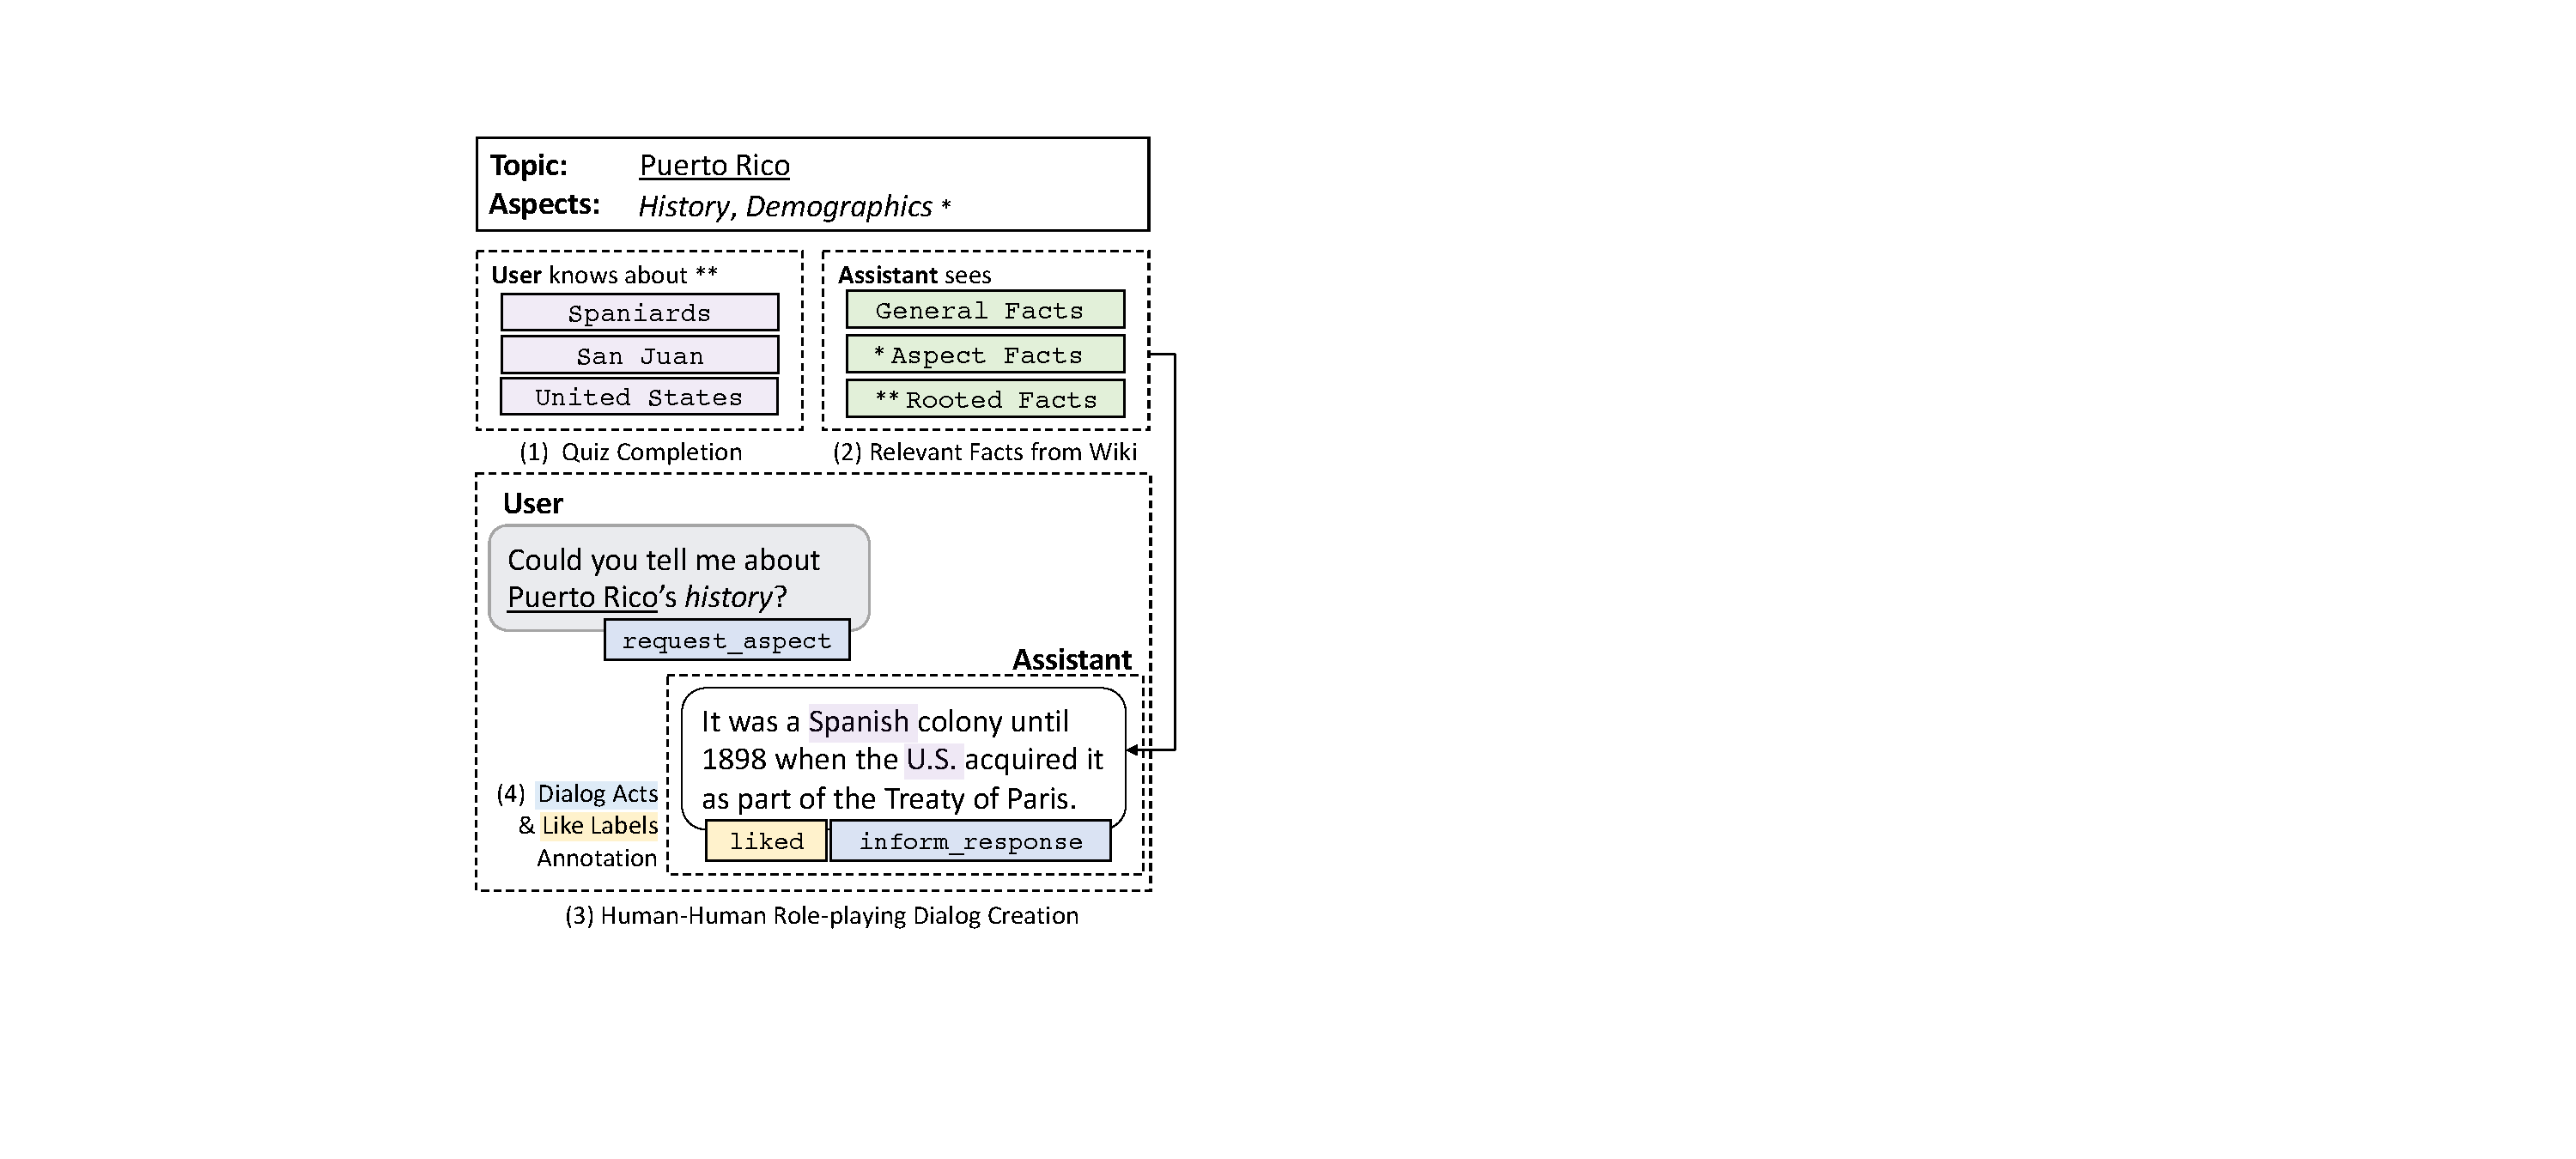
\includegraphics[width=\linewidth]{2020_emnlp_curiosity/figures/rover-dialog}
    \vspace{-16pt}
    \caption{
        We sample pre-existing knowledge by asking users to indicate which \topic{topically} related entities they already \emph{know}.
        The assistant paraphrases facts related to either known entities (rooted facts), an aspect (aspect facts), or the topic generally (general facts).
        The user expresses engagement through a like button.
        Dialog acts are annotated in a separate crowd-source task.
    }
    \vspace{-16pt}
    \label{fig:ex-dia}
\end{figure}

In our dialog task (Figure~\ref{fig:ex-dia}), one worker takes the role of a curious user learning about a geographic entity and the other of a digital assistant with access to Wikipedia facts (Section~\ref{sec:data}).
At the start of each dialog, the user is assigned an entity as their \topic{topic} (e.g., \topic{Puerto Rico}) along with two \aspect{aspects} (e.g., \aspect{history} and \aspect{demographics}) to investigate.
Beforehand, we show the user a list of \entity{entities} related to the \topic{topic}, and they mark which they know; these entities are a sample of their pre-existing knowledge.
The user engages in open-ended discovery while the assistant simultaneously answers the user's questions and proactively introducing facts likely to prompt followup questions.
%For example, if the assistant knew of a user's familiarity with \entity{astronomy} when providing information about \topic{Puerto Rico}, then the user is more likely to engage with and remember facts about the \entity{Arecibo Observatory}.

Section~\ref{sec:analysis} uses dialog act annotations combined with explicit and implicit user feedback to compare assistants' content selection and presentation policies.
For example, in interactions where the user asks a question and the assistant paraphrases a fact, how often does the user ask a followup question versus trail off in disinterest?
Most datasets (Section~\ref{sec:rel}) do not have enough annotations to answer these questions: it requires message-level dialog act annotations and feedback signals.
We compare three assistant policies: using a fact with a rooted entity, a fact from the user's aspect, or a generic fact about the topic.
The policies are compared through user ``likes'' of assistant messages and by the dialog act of their subsequent message~(e.g., did they ask a specific followup or change topic).

In Section~\ref{sec:method}, we design models that predict the policies used by the assistant: what type of message to send and which fact to use~(if any).
All models are trained jointly with a multi-task objective function.
We compare an end-to-end \bert{}~\citep{Devlin2018BERTPO} model to our task-specific Hierarchical Recurrent Encoder model~\citep{Serban2015BuildingED} and show that our model improves over the baseline.

In summary, we make three main contributions: (1) we design an experiment to test the efficacy of personalizing conversational information systems through a user's prior knowledge,  (2) introduce the \rover{} dataset---the first dialog dataset combining sentence-level knowledge groundings, per message ratings, \emph{and} per message dialog act annotations, allowing for robust and fine-grained structural learning of dialog policies for similar applications, and (3) design a multi-task model that incorporates the user's prior knowledge and improves over a natural \bert{} baseline.
